% !TEX root = ../main.tex

\chapter{Recursion proofs}

This chapter serves as an intermediary background exploration, 
diving into more advanced concepts beyond the last chapter's concepts.
Zero-knowledge is dynamic and continuously evolving,
marked by ongoing advancements and active research endeavors. 
Recursion proofs are among the most important and active subjects of these advancements. Recursion proofs are created to accelerate
the generation of multiple zero-knowledge proofs.
Recursion proofs differ in their design. They can vary significantly and serve different use cases.
In this section, we will examine these variations and distinguish between them.
We aim to identify the most suitable method for our daily proof of liabilities and proof of inclusion. \cite{Nova23}


The prover's process in SNARKs is to create a proof using the setup parameters, a private witness, and public input. 
As discussed in the previous section, the proof begins by transforming the code into an arithmetic circuit, 
which is then represented as a polynomial. The polynomial encodes a trace of the circuit (every wire value from inputs to intermediary values to output).
This polynomial is created using the witness (private input).

The objective is to demonstrate that the polynomial satisfies the solution without revealing the polynomial itself. 
This is where the \hyperref[subsec:pc]{polynomial commitment scheme} becomes essential. 
The setup phase generates public parameters that assist in creating and verifying the proof without disclosing the polynomial.

\begin{table}[H]
   \centering
   \caption{Definitions of Symbols in SNARK Circuit}
   \label{tab:snark_symbols}
   \begin{tabular}{|c|p{12cm}|}
   \hline
   \textbf{Symbol} & \textbf{Definition} \\ \hline
   \( S(C) \) & Setup phase that generates the public parameters (\( \text{pp} \) and \( \text{vp} \)) for the prover and verifier. \\ \hline
   \( P(\text{pp}, x, w) \) & Prover function that generates the proof \( \pi \) using the public parameters, public input \( x \), and private witness \( w \). \\ \hline
   \( V(\text{vp}, x, \pi) \) & Verifier function that uses the verification parameters \( \text{vp} \), public input \( x \), and proof \( \pi \) to decide whether to accept or reject. \\ \hline
   \( C(x, w) \) & Arithmetic circuit to generate the polynomial, taking public input \( x \) and private witness \( w \). \\ \hline
   \( w \) & Private witness, representing the prover's secret input. \\ \hline
   \( x \) & Public input, accessible to the prover and verifier. \\ \hline
   \end{tabular}
   \end{table}
   

\begin{figure}[H]
\centering
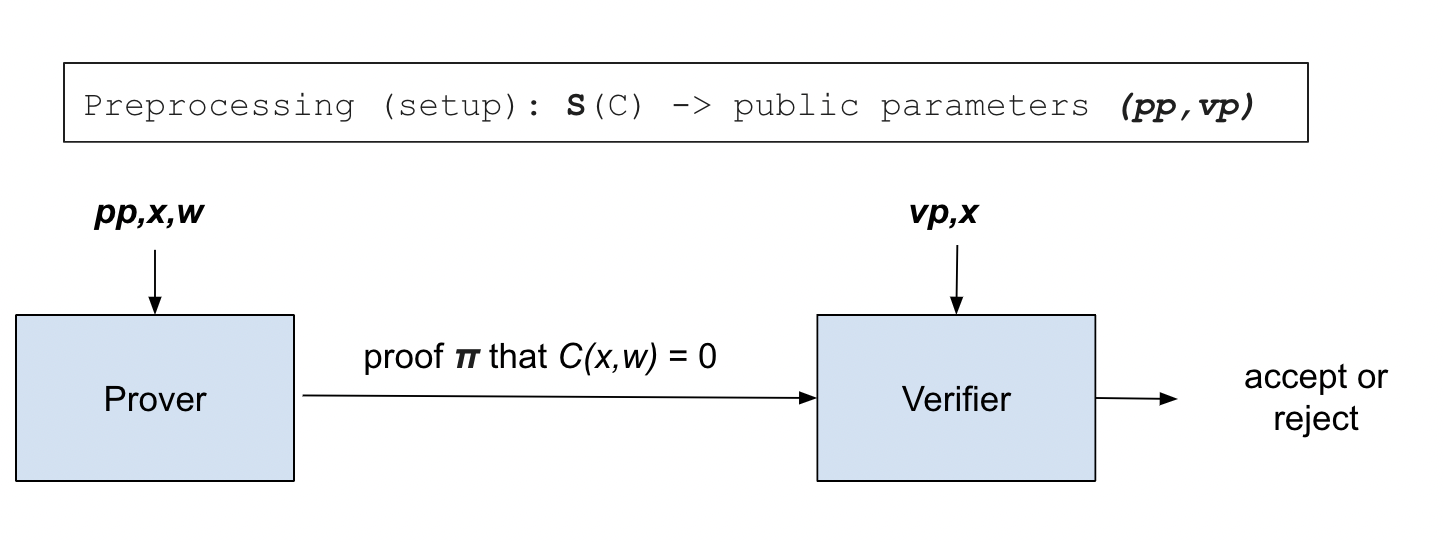
\includegraphics[width=130mm]{SNARKCircuit.png}
\caption{SNARK Circuit \cite{ZKM2}}
\label{overflow}
\end{figure}



\section{Aggregation}
 %-- Can expend on this using \cite{VRS23}, talk about proof composition
 Aggregation is the simplest form of recursion for zk proofs. Its purpose is to reduce the number of proofs that must be verified. 
 It takes a list of proofs as input and outputs a single proof.
 The process involves two phases.
 
 In the first phase, we create our initial proofs.
 In the second phase, these proofs are combined into \verb|"proof of proofs"|. 
 The second phase can be considered a tree, with the initial proofs being the leaves. Each parent node proves the proof of the child nodes.
 The tree can have any number of degrees. We can go from a tree of 2 levels to a binary tree with as many levels as needed.
 
 This is a simple process. Each node has its proof, and then we prove that the other proofs are valid, giving us only one proof
 to verify. Since there are two different phases, two different circuits need to be constructed.
 On the surface, we can parallelize the initial proofs, which decreases the proving time, and we only have one proof to verify, which reduces the verifying time.
 
 However, there are still some aggregation issues.
 The main issue is that a verification circuit is more complex than a proof of transaction.
 Verifying a proof involves constructing a circuit to represent the verification process itself, which is inherently complex. 
 This circuit must perform cryptographic operations, including curve arithmetic and bilinear pairings, which must be implemented directly at the circuit level. 
 As a result, the verification circuit is essentially the exponent of the cryptographic process.
 This becomes a scaling issue since the proof time of the second circuit grows linearly with the number of proofs to verify. \cite{Nova23}
\iffalse
\begin{figure}[H]
 \centering
 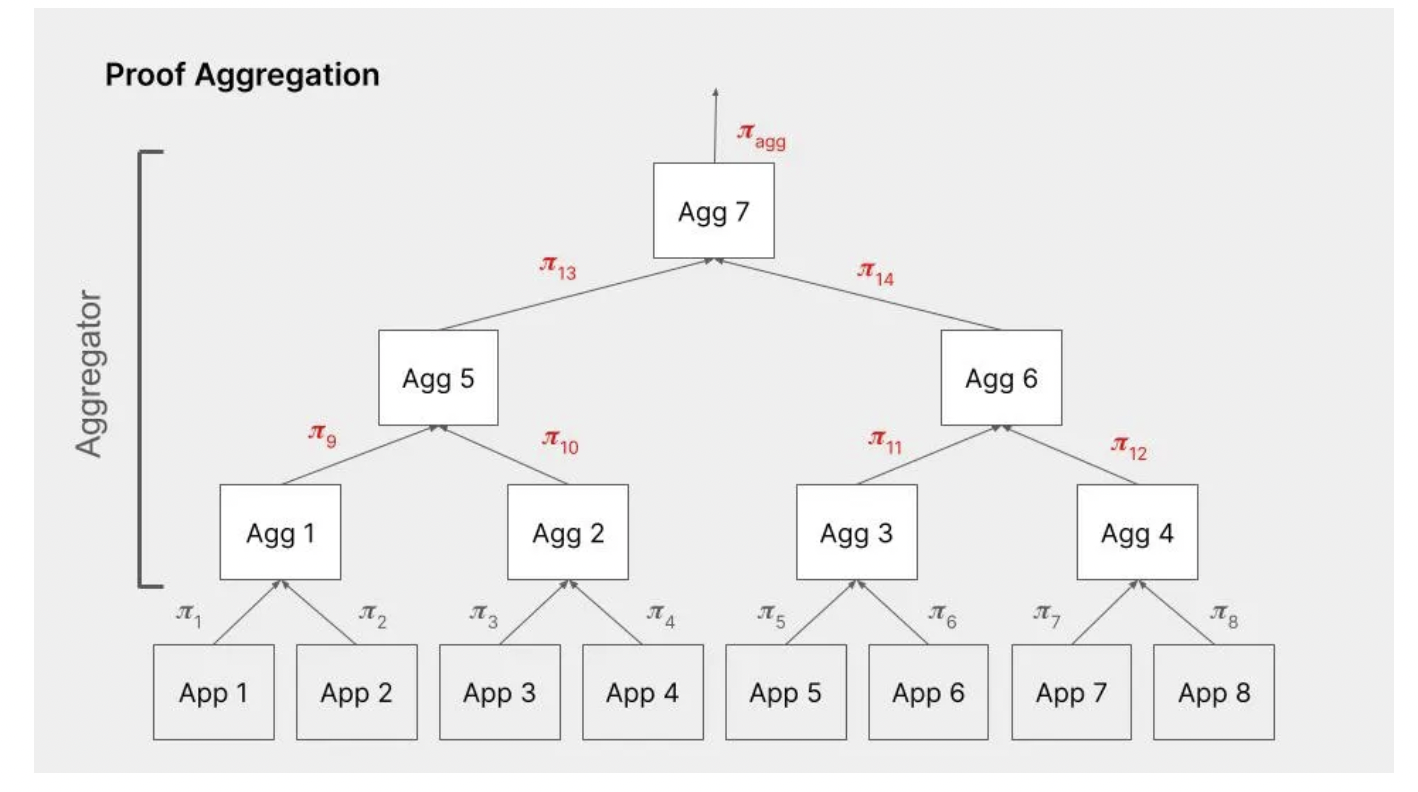
\includegraphics[width=130mm]{AggregationProof.png}
 \caption{Aggregation Proof \cite{TP24}}
 \label{overflow}
 \end{figure}
\fi

\section{Recursion scheme}
The following technique is the recursion scheme, or Incrementally Verifiable Computation (IVC). Like the aggregation, the proof is separated into nodes.
However, in this case, each node serves two purposes: to prove that the node itself is valid and that the previous proof is valid.
The number of constraints will always stay the same because it only proves two things of fixed sizes. This creates
a chain structure, where verifying the latest node is the equivalent of verifying every node in the chain.
It is an improvement from the previous technique for two reasons.
First, this allows the maintenance of a constant number of constraints in the circuit.
Second, we do not have to redo a trusted setup once the proof size is defined.
This means the trusted setup remains the same; we do not have to redo it.
This implies that the latest node does not take longer to verify than the second node.
However, each node still has to verify the previous node, which takes additional time. \cite{Nova23}


\section{Accumulation}
Accumulation schemes offer a different approach to aggregating proofs than IVC. 
Instead of verifying proofs at each step, accumulation defers all heavy computational tasks to the final step.
This allows proofs to be efficiently added to an accumulator while minimalizing the intermediate verification workload. 
Each step adds a new proof to the accumulator while maintaining a small and constant-sized state. 
Unlike recursion, where each proof is verified within the circuit immediately, accumulation schemes delay all verification until the final stage, 
where all accumulated proofs are checked simultaneously.

There are different types of accumulation schemes, each handling proof accumulation in a distinct way.
Some, like polynomial accumulation, track commitments to polynomial evaluations over multiple steps. 
Others, such as accumulation based on cryptographic accumulators (e.g., RSA or Merkle accumulators), focus on aggregating statements into a compact structure. 
Regardless of the method, the core idea remains the same: verification is deferred to the final proof, preventing the verification cost from increasing with each step.

Accumulation schemes relate to Incrementally Verifiable Computation (IVC) because both aim to make verifying long computations more efficient. 
However, the key difference is that IVC requires each step to verify the previous one while keeping proof sizes constant, while accumulation postpones all verification until the final step. 
This makes accumulation more suitable for cases where verifying everything at the end is preferable to verifying at every step.

The advantage is clear: instead of paying the cost of verification $n$ times throughout the process, we pay it once at the end. 
This is especially useful when multiple independent proofs need to be efficiently combined without introducing the recursive overhead of IVC. 
However, this benefit comes with a tradeoff. Since all verifications are deferred, the final step can be computationally expensive.\cite{BB20}


\subsection{Halo accumulation}
The concept of deferring the polynomial commitment opening and consolidating them into a single operation was introduced by Bowe, Grigg, and Hopwood Halo.\cite{BGH23}
This process involves two parts:
The first part is fast, where we output a polynomial and its commitment.
The second part is expensive. In it, we verify the pair $(f_1, c_1)$ of the polynomial $f_1$ and its commitment $c_1$. We open the polynomial only at a specific point.
The second part can be accumulated if the commitment scheme is additively homomorphic. 
Instead of individually verifying each pair, we accumulate the pairs and verify their linear combinations ($c_1+c_2+...$ is a commitment for $f_1+f_2+...$). \cite{VR23}


\section{Folding scheme}
In the Nova scheme, the folding technique accumulates the R1CS progressively as the computation proceeds rather than accumulating only the complex portions of the R1CS. 
This means that at each step in the folding process, instead of storing the separate R1CS sets for each node and combining them later, we incrementally combine them into a single R1CS set. 
This set, called "relaxed R1CS," simplifies the final proof generation.
As a result, we avoid the need to handle multiple sets of R1CS in the final step, leading to a more efficient recursive proof process. 
The relaxed R1CS is then used to compute a single proof at the end of the folding process.
\cite{Nova23}  \cite{ASI23} \cite{vODC24F}

\subsection{Relaxed R1CS}
Returning to the previous \hyperref[subsec:r1cs]{section}, we previously defined what an R1CS is.
The goal is to combine 2 R1CS and obtain another R1CS. If we succeed, we can fold every R1CS together and be left with only one.


If we \textbf{define our R1CS}:
\begin{quote}
\textbf{fix an R1CS} program $A,B,D \in \mathbb{F}^{u \times v}_p $
\\
We define $x$ as the public input and $w$ as the witness.
\\
Instance 1: $ x_1 \in \mathbb{F}^n_p $, $ z_1 = (x_1, w_1) \in \mathbb{F}^v_p$
\\
Instance 2: $x_2 \in \mathbb{F}^n_p $, $ z_2 = (x_2, w_2) \in \mathbb{F}^v_p$
\\
Where $u$ is the number of constraints in the R1CS, $v$ is the number of variables in the constraint system, $p$ is the private field, and $n$ is the number of public variables.
\\
We know $Az_i \circ Bz_i = Dz_i$ for $ i = 1,2$
\end{quote}


\textbf{Recall}: Our R1CS must be valid for any field element.
To prove this, the verifier chooses a random point $r$ at which we will evaluate our constraints system.

The naïve approach to folding an R1CS is to sum the two instances together.

\textbf{First attempt}:
\begin{quote}
Let us define $r$ as a random variable:
\\
$r \leftarrow \mathbb{F}_p$
\\
Then we set 
\\
$x \leftarrow x_1+rx_2$
\\
$z \leftarrow z_1 + rz_2 = (x_1+rx_2, w_1 + rw_2)$
\end{quote}


Then:
\begin{quote}
   $Az \circ Bz = A(z_1 + r z_2) \circ B(z_1 + rz_2)$
   \\
   $= (Az_1) \circ (Bz_1) + r^2 (Az_2) \circ (Bz_2) + (r(Az_2) \circ (Bz_1) + r(Az_1) \circ (Bz_2))$
   \\
   $=Dz_1 + r^2Dz_2 + E$
   \\
 Where $E$ is a combination of the remaining values.
   \\
\end{quote}

Simply summing the constraints does not preserve the R1CS structure we just defined: $Az_i \circ Bz_i = Dz_i$.
Since the direct addition of two R1CS instances does not produce another valid R1CS, we need a different approach.

We need to modify the R1CS so that it can be folded.
To solve this, we introduce a relaxed R1CS, which includes a new error term $E$.
The goal is to have the new terms produced by the folding comprised in the term $E$.
We will try the new form: $Az_i \circ Bz_i = Dz_i Ez_i$.
\\
\\
Let's \textbf{define a relaxed R1CS}:
\begin{quote}
$A, B,D \in \mathbb{F}^{u \times v}_p, (x \in \mathbb{F}^n_p, c \in \mathbb{F}_p, E \in \mathbb{F}^u_p) $
\\
Witness: $ z = (x,w) \in \mathbb{F}^v_p s.t. (Az) \circ (Bz) = c(Dz) + E$
\end{quote}
Lets \textbf{fix the R1CS} program once again:
\begin{quote}
$A,B,D \in \mathbb{F}^{u \times v}_p $
\\
Instance 1: public $ (x_1,c_1,E_1)$, witness $z_1 = (x_1, w_1) \in \mathbb{F}^v_p$
\\
Instance 2: public $(x_2,c_2,E_2)$, witness $ z_2 = (x_2, w_2) \in \mathbb{F}^v_p$
\\
We know $(Az_i) \circ (Bz_i) = c_i(Dz_i) + E_i$ for $ i = 1,2$
\end{quote}


\textbf{Second attempt}:
\begin{quote}
$T \leftarrow (Az_2) \circ (Bz_1) + (Az_1) \circ (Bz_2) - c_1(Dz_2) - c_2(Dz_1)$
\\
$x \leftarrow x_1 + rx_2, c \leftarrow c_1 + rc_2, E \leftarrow E_1 + rT +r^2E_2$
\\
$z \leftarrow z_1 + rz_2 = (x_1 +rx_2, w_1 + rw_2)$
\\
$Az \circ Bz = $
\\
$=A(z_1) \circ rB(z_1) +r^2(Az_2) \circ (Bz_2) + r(Az_2) \circ (Bz_1) + r(Az_1) \circ (Bz_2)$
\\
$=c_1(Dz_1) + E_1 + r^2c_2(Dz_2) + r^2E_2+r((Az_2) \circ (Bz_1) + (Az_1) \circ (Bz_2))$
\\
$=(c_1+rc_2)(Dz_1+rDz_2)+E_1+r^2E_2+rT$
\\
$=c(Dz) + E$
\end{quote}
We have a valid relaxed R1CS.

\paragraph{Validity}
While the error term $E$ allows folding, it questions the validity of the proof. As long as $E$ is bounded, the proof remains valid. 
The relaxed formulation preserves constraint structure, enables incremental folding, and prevents uncontrolled error propagation. 
If needed, the system can return to a strict R1CS by proving $E = 0$ in the final verification, ensuring flexibility and correctness.
\cite{Nova23}